\section{Adding a barrier to the box-potential}
Let us now consider a potential barrier in the box, modeled by the dimensionless potential $\nu(x') = t_0V_0/\hbar$, where $t_0 =\frac{2mL^2}{\hbar}$ as in \cref{eq:normalized_stuff}, and is given by
\begin{equation} 
\nu(x') = \begin{cases}
0,\quad &0<x'<\frac{1}{3} \\
\nu_0 = \frac{2mL^2V_0}{\hbar^2},\quad &\frac{1}{3}<x'<\frac{2}{3} \\
0,\quad &\frac{2}{3}<x'<1 \\
\infty ,\quad &\text{otherwise}
\end{cases}
\end{equation}
Thus, setting $\nu_0$ to 0 is the same task as we had for the previous case, since we have the same boundary conditions and a vanishing potential between the edges, which ensures that the matrix-representation (and thus the eigenvalues) of the operator acting on the wave function is equal. 
Now we set $\nu_0 = 10^3$.
Comparing the energy eigenvalues for the problem, we find that some seem to be equal, i.e. there seems to be degeneracy in the system. This cannot be, since we are in 1D with a discrete energy spectrum \cite{hemmer1985kvantemekanikk}. Indeed, the states are equal, as we can see for the lowest lying energy eigenfunctions in \cref{fig:degeneracy}.
\begin{figure}
	\centering
	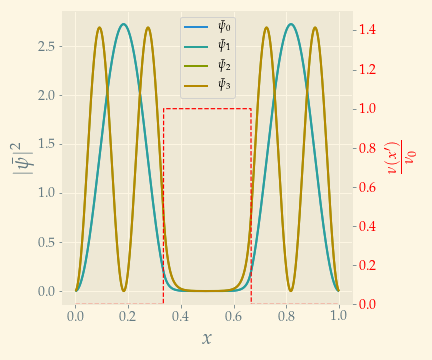
\includegraphics[width=\linewidth]{img/degeneracy.png}
	\caption{Degeneracy of the ground state and first excited states plotted together with the potential.}
	\label{fig:degeneracy}
\end{figure}
We now prepare the initial state 
\begin{equation} 
\label{eq:psi0}
\Psi_0 = \frac{1}{\sqrt{2}}\left( \psi_1(x') + \psi_2(x') \right)
\end{equation}
and let it evolve from $t_0'=0$ to \begin{equation}
\label{eq:time}
t_1'=\frac{\pi}{\lambda_2 -\lambda_1},
\end{equation}we find that the particle has tunneled from one side of the barrier to the other! This is shown in \cref{fig:tunneling}. 
\begin{figure}[tb]
	\centering
	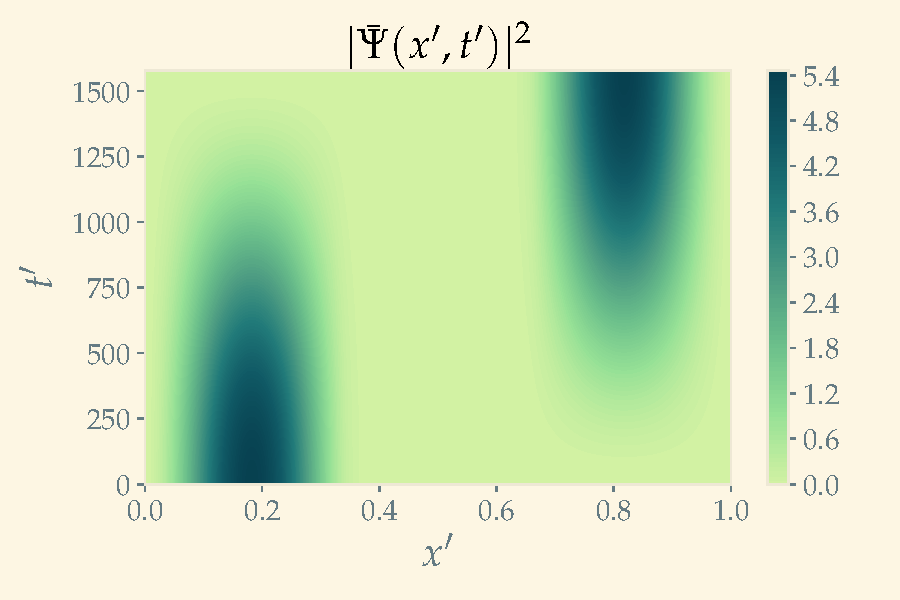
\includegraphics[width=\linewidth]{img/tunneling.pdf}
	\caption{Tunneling across the potential barrier.}
	\label{fig:tunneling}
\end{figure}
We can see that the initial state (on the left side of the potential barrier) ``leaks'' into the opposite side as time progress. Inserting \cref{eq:time} into \cref{eq:full_state}, we find (after some manipulation) 
\begin{equation} 
\Psi(x', t'_1) = C\left(\psi_2(x')-\psi_1(x')\right)
\end{equation}
for a normalization constant $C$. 
This is the initial state mirrored about $x' = 1/2$.
